\documentclass[a4paper, 12pt]{article}

\usepackage[utf8]{inputenc}

%images
\usepackage{graphicx}       %for inserting images
\graphicspath{./images/}    %image file directory
\usepackage{wrapfig}
%caption
\usepackage{caption}
\captionsetup{
   font=small,
   labelfont=bf,
   tableposition=top
}
%page margins, geometry
\usepackage{geometry}
\geometry{margin = 1in}

%headers and footers
% All page numbers positioned at the bottom of the page
\usepackage{fancyhdr}
\fancyhf{} % clear all header and footers
\fancyfoot[C]{\thepage}
\renewcommand{\headrulewidth}{0pt} % remove the header rule
\pagestyle{fancy}

%for inserting columns
\usepackage{multicol}       
\setlength{\columnsep}{1cm}

%bibilography
\usepackage{biblatex}
\addbibresource{biblography.bib}

%to use sample texts
\usepackage{blindtext}


\begin{document}

\begin{center}
     \textsc{\Huge {Drive Motor Requirements\\}}
\end{center}

%document authors 
\begin{center}
\begin{tabular}{c c c c}
     \textsc{Y.S. Ginige} & 180195A &  \textsc{P.M.P.H. Somarathne} & 180616T\\
     \textsc{V.Y.N. Lokugama }& 180359G & \textsc{A. Thieshanthan} &  180641N\\
       \textsc{W.A.V. Ravihansa} &  180544U &  \textsc{L.T.N. Wickremasinghe} & 180701B
\end{tabular}
\end{center}

%abstracct

%content after this

\normalsize
\subsection*{Robot Total Weight Calculation}
\begin{center}
    

\begin{tabular}{|c |c|}
\hline
Component & Weight \\
\hline
Lipo Batteries – 200g x 2    & 400g \\
Arduino mega          &                        40g\\
12V motors – 200g x 2    &                         400g\\
Arduino nano   &                                  7g\\
OLED Display            &                                    15 g\\
Dangaya Motor Controller   &                   75g\\
Servo motors – 20g x 3     &                       60g\\
Color Sensors – 15g x 2   &                       30g\\
ToF and Gyro meter     &                      20g\\
Wheels, Spaces, Nuts       &                    80g\\
Raykha Sensor              &                        25g\\
Perspex floors             &                       100g\\
Wires and other        &                      50g\\
Body Cover             &                       100g \\
\hline
\textbf{Total Weight (Worst case)}        &       \textbf{1500g}\\
\hline
\end{tabular}
\end{center}

\subsection*{Motor Specification Calculation}

According to the path that robot is going to follow, the highest current and the torque will be needed at the ramp sub-task. Worst-case scenario will be, robot stopping at the ramp-start and trying to climb it. This case will require the highest torque and current. \par

We do the calculations for starting the ramp at zero speed and accelerating to $6cms^{-1}$ in 2s. Then climb the rest with that constant speed.\\
\\
Accelerated distance = \begin{Large}$\frac{(V+U)\times2}{2}$\end{Large} = $6 cm$\\
\\
Then, we can do the ramp climb in $2 + 38/6 = 8.3 s$.\\
\\
Acceleration =  $6/2 = 3cms^{-2}$\\
\begin{figure}[h]
    \centering
    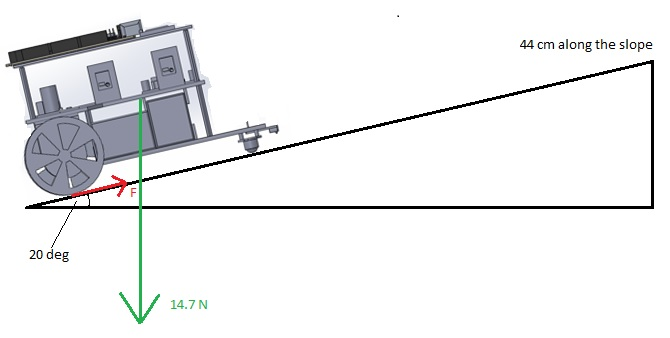
\includegraphics[scale = 0.8]{images/WhatsApp Image 2020-05-07 at 13.20.09.jpeg}
    \caption{Free body diagram for robot on the ramp.(Only the forces which affect the ascend are marked here)}
    \label{fig:my_label}
\end{figure}
By applying $F=MA$ to the robot along the inclined plane.\\
\begin{tabular}{l l}
  Total force needed by wheels   & $ = mg sin(20) + mA$\\
			                     & $= 1.5\times9.8\times sin(20) + 1.5 \times 3/100$\\
			                   &  $= 5.077 N$\\ 
     
\end{tabular}\\
Force required by one wheel $= 5.077/2 = 2.54 N $\\
Radius of the wheel $= 3cm$\\
\begin{tabular}{l l}
     Torque required from a wheel &$ = Fd$\\
			            &$= 2.54 \times 3 Ncm$\\
			            &$= 7.62 Ncm$  \\    
			            &$= 0.777 kgcm$\\
\end{tabular}
\\
\\      
To leave a 25\% space for any error (friction), We should use a motor with \textbf{1.036 kgcm} stall torque at least.\\

\begin{tabular}{l l}
   Angular Velocity at the maximum speed in the ramp & $= 6 cms^{-1}/ 3 cm$\\
						         &$= 2 rads^{-1}$\\
						        &$= 19.1 rpm$\\
\end{tabular}\\
\begin{tabular}{l l}
Maximum power output of the motor (P) & $= \tau \omega $\\
							   &$= 7.6 \times 2 / 100 Nm$\\
							   &$= 0.144 W$\\
\end{tabular}

\subsection*{Descend from the Ramp}
To maintain a constant speed, again motors should take the torque generated by weight.\\
\\
Torque = \begin{Large}$\frac{1.5\times 9.8 \times sin(20) \times 3}{2}$\end{Large} Ncm = $7.54\ Ncm = 0.76\ kgcm$\\
\\
$\omega$ = \begin{Large}$\frac{44 cm}{10\ s \times 3\ cm}$\end{Large} = $1.5\ rads^{-1}$\\
\\
Power required during the descend = \begin{Large}$\frac{7.54 \times 1.5}{100}$\end{Large} = $0.11\ W$
\subsection*{On flat ground}
We are planning to complete the first line following part (approximately 250 cm) in 30 seconds and it will be the fastest run.\\
\\
Maximum RPM needed = \begin{Large}$\frac{250 \times 60}{30 \times 2\pi \times 3}$\end{Large} = $26.52\ rpm$\\
\\	
\textbf{Selected motor:} Pololu 25D 12V high power 47:1 gear motor with encoders.

Stall Torque = $8.64\ kgcm\ @9V$

Stall Current = $4.2\ A\ @9V$

\end{document}
